\question{9.7}{
    Capsules die zijn gevuld met een bepaald medicijn, moeten $5$ mg werkzaam bestanddeel bevatten.
    Het is bekend dat door onnauwkeurigheden met de machine die de capsules vult de hoeveelheid werkzaam bestanddeel te beschouwen is als een normaal verdeelde kansvariabele $X$ met verwachtingswaarde $5,0$ mg en standaarddeviatie $0,15$ mg.
    Ge\"eist wordt dat de hoeveelheid werkzaam bestanddeel per capsule tussen $4,6$ en $5,4$ mg ligt.
}
\begin{enumerate}[label=(\alph*)]
    \item Hoeveel procent van de capsules heeft een inhoud buiten de gestelde normen als de vulmachine correct is ingesteld?
    \answer{
        Gegeven is dat de hoeveelheid (in mg) werkzaam bestanddeel $X \sim N(\mu=5,0; \sigma=0,15)$.
        De norm is dat deze hoeveelheid tussen de $4,6$ en $5,4$ mg ligt.
        De kans hierop kunnen we uitrekenen als volgt:
        \begin{align*}
            P(4,6 \le X \le 5,4) = \normalcdf(a=4,6; b=5,4; \mu=5,0; \sigma=0,15) \approx 0,9923
        \end{align*}

        Met $99,23\%$ kans wordt een willekeurige capsule gevuld met een hoeveelheid werkzaam bestanddeel dat binnen de norm valt, oftewel $0,77\%$ van de capsules heeft een inhoud buiten de gestelde normen.
    }

    \item De instelling van de machine kan tijdens het gebruik veranderen.
    Daarom wordt er regelmatig een aantal capsules gecontroleerd in het laboratorium.
    Een steekproef van $25$ capsules levert een gemiddeld gehalte van het werkzame bestanddeel van $4,70$ mg.
    Toets of hieruit mag worden geconcludeerd dat de instelling van de machine is gewijzigd.
    Toets hierbij tweezijdig, kies $\alpha=0,01$ en ga ervan uit dat de standaarddeviatie niet is veranderd.
    \answer{
        In deze hypothesetoets geldt dat de nulhypothese $H_0: \mu = 5,0$ (geen verandering in de instelling) getest wordt tegen de alternatieve hypothese $H_1: \mu \neq 5,0$ (wel een verandering in het gemiddelde).
            
        Omdat we tweezijdig toetsen, berekenen we de $z$-waarde
        \[
            z_{\alpha/2} = \invnorm(opp=1-\alpha/2) = \invnorm(opp=0,995) \approx 2,5758
        \]

        De toetsingsgrootheid is weer het (theoretische) steekproefgemiddelde $\overline{X}$.
        Uit de centrale limietstelling volgt dat $\overline{X} \sim N(\mu; \frac{\sigma}{\sqrt{n}})$.
        Onder de aanname dat $H_0$ waar is, geldt dat het gemiddelde $\mu = 5,0$.
        Verder geldt dat de standaardafwijking $\sigma = 0,15$ bekend is en dat er $25$ capsules worden getest, oftewel de steekproefomvang $n=50$.
        Er volgt dus dat $\sigma(\overline{X}) = \frac{\sigma}{\sqrt{n}} = \frac{0,15}{\sqrt{25}}=0,03$, oftewel $\overline{X} \sim N(\mu=50; \sigma=0,03)$.
        Merk op dat hoe verder het steekproefgemiddelde afligt van $5,0$ (zowel ver daaronder als ver daarboven), hoe waarschijnlijker dat de alternatieve hypothese waar is.
        Het kritieke gebied is dus van de vorm $(-\infty, g_1]$ en $[g_2, \infty)$, waarbij $g_1$ en $g_2$ kunnen worden berekend als volgt:
        \begin{align*}
            g_1 &= \mu - z_{\alpha/2} \cdot \frac{\sigma}{\sqrt{n}} \\
                &= 5,0 - 2,5758 \cdot \frac{0.15}{\sqrt{25}}\\
                &\approx 4,9227 \\
            g_2 &= \mu + z_{\alpha/2} \cdot \frac{\sigma}{\sqrt{n}} \\
                &= 5,0 + 2,5758 \cdot \frac{0.15}{\sqrt{25}} \\
                &\approx 5,0773 \\    
        \end{align*}

        Het kritieke gebied is dus gelijk aan $(-\infty; 4,9227]$ en $[5,0773, \infty)$.
        Het geobserveerde steekproefgemiddelde $\overline{x}=4,70$ ligt in het kritieke gebied, dus we verwerpen $H_0$.
        Er is voldoende reden om aan te nemen dat de instelling van de machine is gewijzigd. 

        \begin{center}
            \resizebox{0.9\textwidth}{!}{
                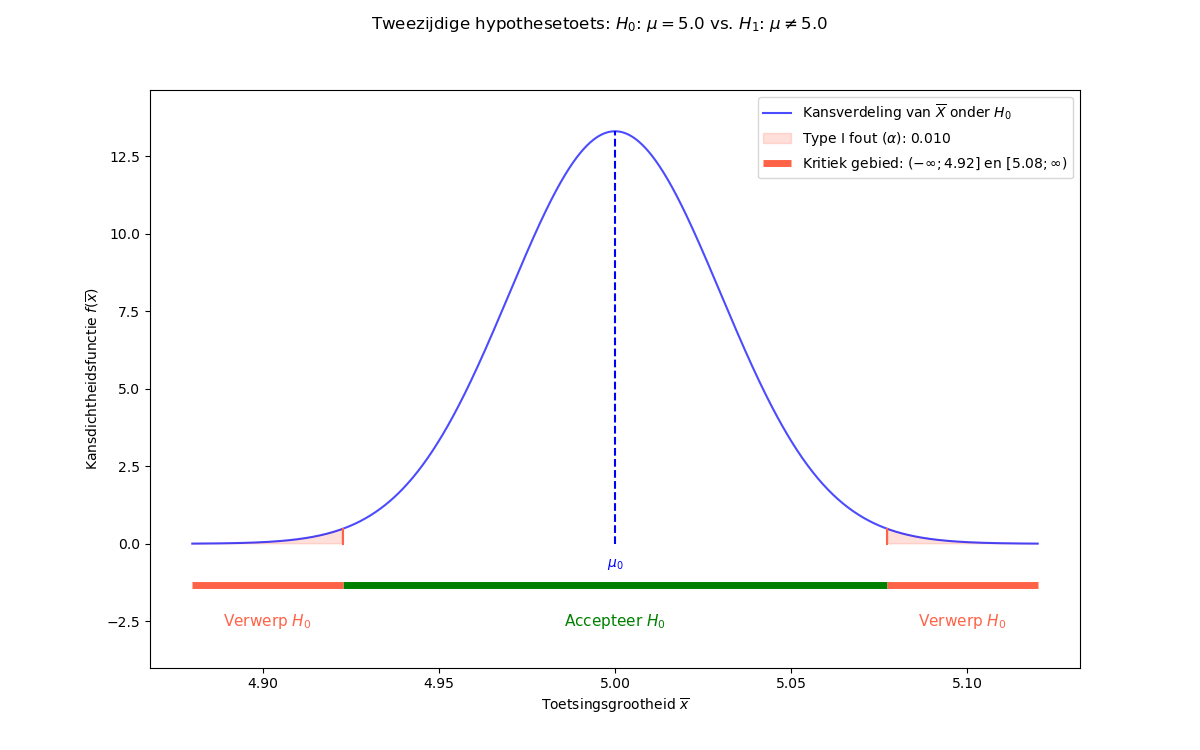
\includegraphics{opg_9.7b.png}
            }
        \end{center}
    }

    \item Als de capsules worden gevuld met gemiddelde $4,70$ mg werkzaam bestanddeel ($\sigma$ is nog steeds gelijk aan $0,15$ mg), hoeveel procent van de capsules voldoet dan niet meer aan de norm?
    \answer{
        Stel nu dat het gemiddelde $\mu = 4,70$ mg, en de standaarddeviatie is nog steeds $\sigma = 0,15$, oftewel $X \sim N(\mu=4,70; \sigma=0,15)$.
        In dat geval is de kans dat een willekeurige capsule niet meer voldoet aan de norm gelijk aan
        \begin{align*}
            P(4,6 \le X \le 5,4) = \normalcdf(a=4,6; b=5,4; \mu=4,7; \sigma=0,15) \approx 0,7475
        \end{align*}
        $74,75\%$ van de capsules zal nu een hoeveelheid werkzaam bestanddeel bevatten dat voldoet aan de norm, oftewel $25,25\%$ van de capsules voldoen niet aan de norm.
    }
\end{enumerate}